\subsection{Beleuchtung}
\label{subsec:Beleuchtung_2}

Damit die Maschine von weitem erkennbar ist und auch Eindruck schindet, eignet sich ein LED-Band. Am Besten, wenn es noch verschiedenfarbig ist. Der Aufbau eines LED-Bandes ähnelt dann dem in Abbildung \ref{fig:LED1} gezeigten Schaltung. Der Streifen ist Rot eingerahmt, die LED's und Widerstände befinden sich auf dem Band und die zu sehenden Fähnchen für R, G, B und W führen über die Leistungs-MOSFETS. Die MOSFETs wiederum werden vom Mikrocontroller angesteuert.

\begin{figure}[H]
\center
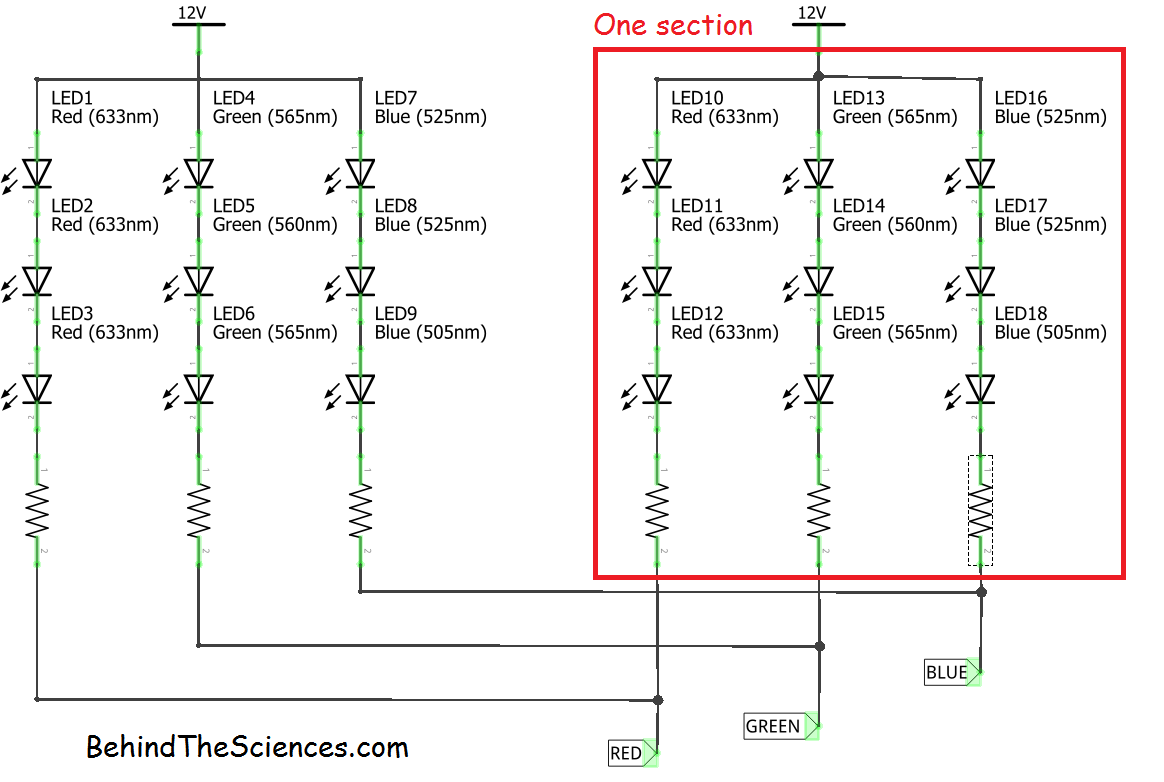
\includegraphics[width = 0.5\textwidth]{graphics/Schema_LED1}
\caption{LED Beispiel. \cite{behindthesciences_rgb_2017}}
\label{fig:LED1}
\end{figure}

\paragraph{Schema}\mbox{}

Bei Licht handelt es sich um elektromagnetische Wellen, welche im sichtbaren Wellenlängen-Bereich liegen. Dabei gibt es vier Hauptfarben: Rot, Grün, Blau und Weiss. Zwar kann Weiss auch aus einer Kombination aller drei Farben erstellt werden, es kommt aber besser mit einer separaten Diode. Das resultierende Licht des Bandes ist eine Überlagerung der Wellenlängen. Diese Überlagerung kann vom Mikrocontroller über den Duty-Cycle eines PWM-Signals gesteuert werden. So lassen sich mit dem Licht aus den Grundfarben praktisch alle Farben mischen. Abbildung \ref{fig:Schema_LED} zeigt den Schaltungsaufbau der LED-Steuerung mit den MOSFETs und zugehörigen passiven Bauteilen.

\begin{figure}[H]
\center
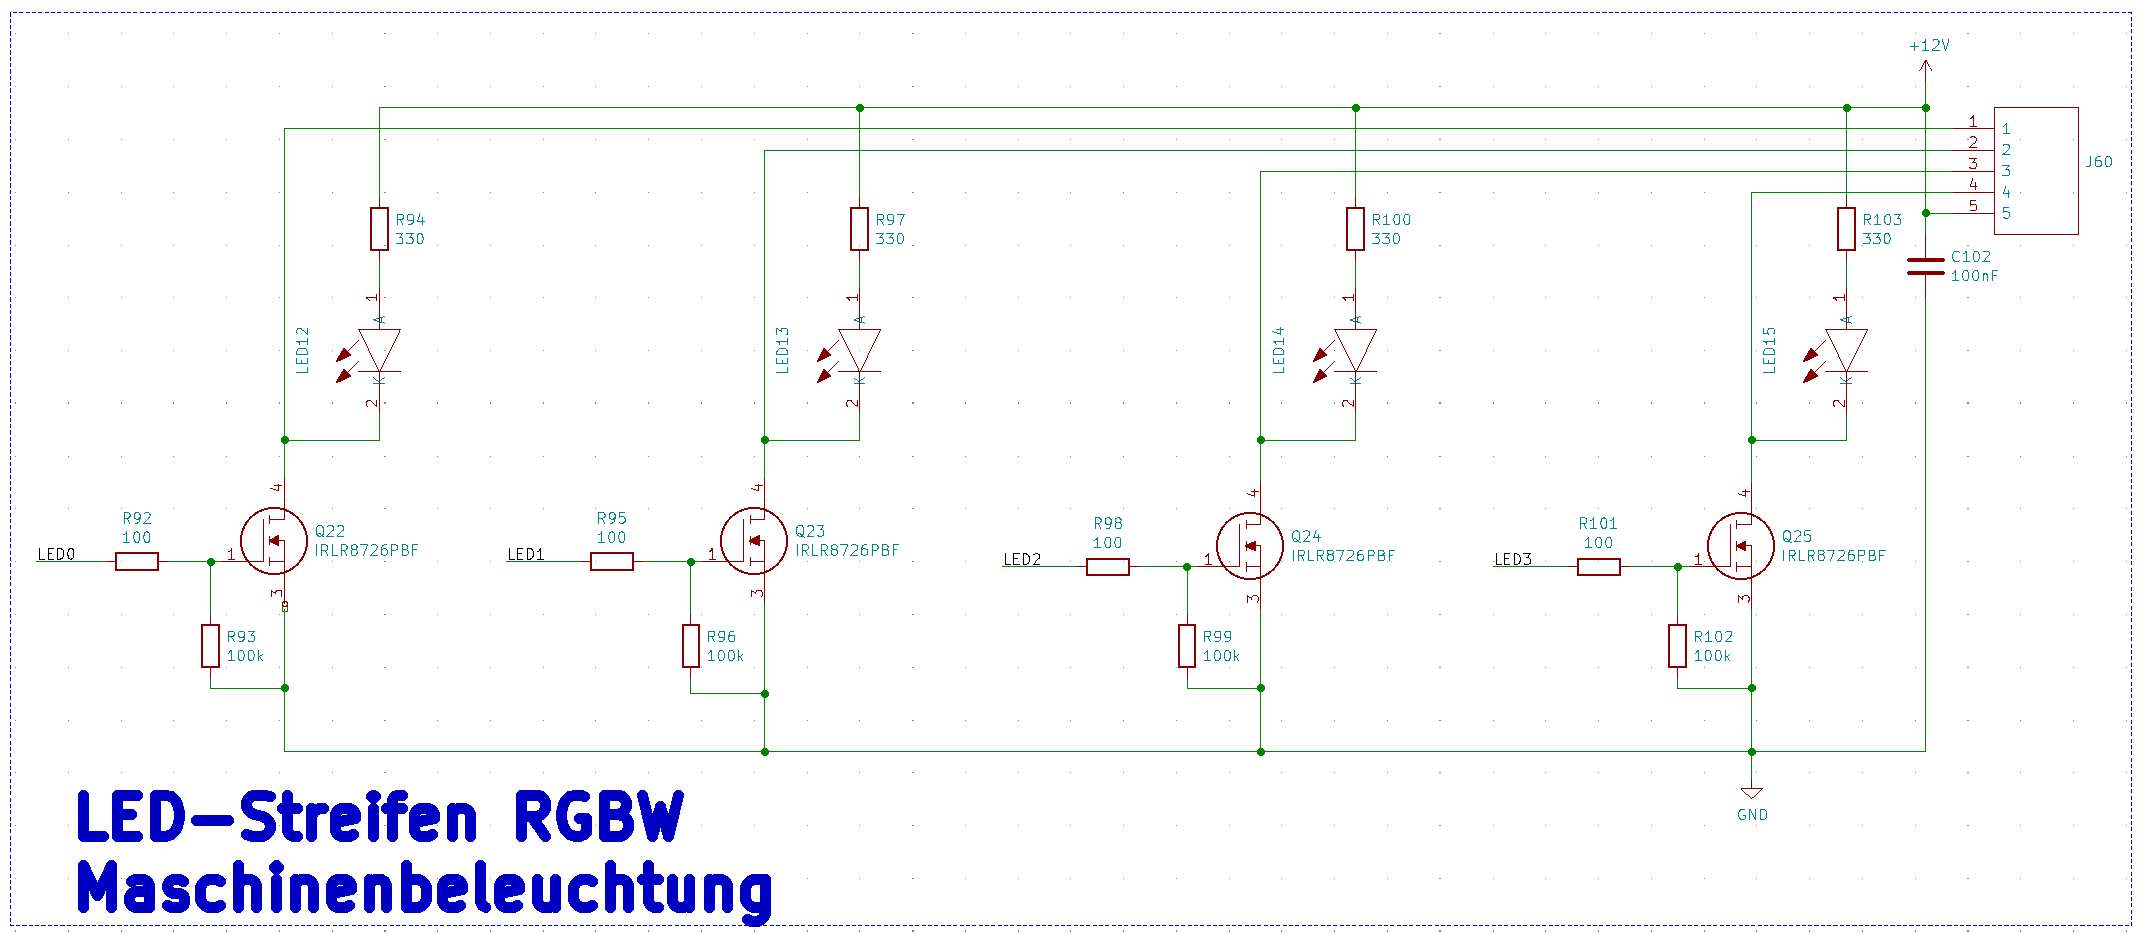
\includegraphics[width =  \textwidth]{graphics/Schema_LED}
\caption{Schema der LED-Ansteuerung}
\label{fig:Schema_LED}
\end{figure}

\paragraph{Funktionsbeschrieb der Schaltung}\mbox{}

Damit die LED's angesteuert werden können, braucht es ein Bauteil welches mit einer 5V-Eingangssignal 12V schalten können. Dazu wird der selbe MOSFET Q22 bis Q25 verwendet wie schon bei den Pumpen in Kapitel \ref{subsubsec:Pumpen}. Über die Widerstände an den Gates wird der Strom zum Schutz des Gates begrenzt. Ausserdem verhindern sie ein allfälliges Oszillieren. Die Leitungen führen direkt auf den Klemmblock für die LED-Streifen. Die parallel geschalteten LEDs LED12 bis LED15 sind zum Debuggen ohne LED-Streifen.